\section{Approach}

We took three approaches to improve the performance of our model against the baseline Alexnet~\cite{alexnet} model trained with the example code. First, we trained newer, smaller, network architectures on the training set including Inception~\cite{inception} and ResNet~\cite{resnet}. Second, we augmented our training data to reduce overfitting during training by altering the image properties (color, brightness, etc), taking a random sub-image, and flipping the image vertically. Finally, we ensembled our best performing models together with a range of techniques described in detail in Section~\ref{s:experiments}. Using these three methods together yielded the best results on our validation set.

\subsection{Network Architectures}
With the baseline AlexNet code, we were able to achieve about 70\% top-5 accuracy. We felt that with newer model architectures, it would be possible to achieve higher performance. We settled on two models, ResNet V2 101 and Inception V3. Even with fewer parameters these architectures are shown to perform better on the Imagenet~\cite{imagenet} classification task~\cite{model-comparison}. We reasoned that these architectures may also perform well on the Miniplaces task compared to AlexNet without a significant impact on training time. Inception is a deep network architecture made up of many stacked inception modules, as seen in Figure \ref{fig:inception-module}. Inception allows for the expressibility of some 5x5 convolutions without forcing the entire layer to consist of these large convolutions, this saves parameters without giving up expressibility. We also trained a ResNet model. ResNet forwards the output of some layers forward in the network, and adds them together. Effectively this means that during backpropagation the gradients from some subsections of the network can be passed back to earlier layers of the network without going through intermediate layers. This can be seen in the ResNet block in Figure \ref{fig:resnet-block}. Another advantage of both Inception V3 and Resnet is a single fully connected layer compared to AlexNet's two, reducing the number of parameters required. We trained these networks with standard batch normalization and dropout techniques. 

\begin{figure}[b]
\centering
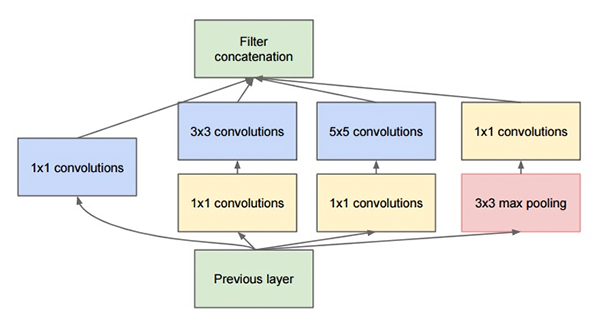
\includegraphics[width=\columnwidth]{figures/inception_module}
\caption{Single Inception~\cite{inception} module}
\label{fig:inception-module}
\end{figure}

\begin{figure}[b]
\centering
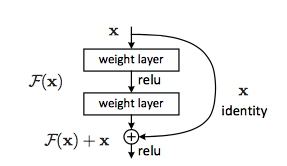
\includegraphics[width=\columnwidth]{figures/residual_block}
\caption{Single Resnet~\cite{resnet} block}
\label{fig:resnet-block}
\end{figure}

\subsection{Data Augmentation}
In the course of training our models, we found that many of the models overfit our training data, achieving near perfect top-1 accuracy on the the training set, but had 10s of percentage points worse accuracy on the validation set. We reasoned that the model was 'memorizing' the training set and not generalizing well. Even at best, the models accuracy on the validation set was around 70\%.We augmented our dataset using four techniques; perturbing image properties, mirroring the image, and taking a random subimage. Each of these operations is performed randomly at training time by taking an image and perturbing it with a random order of the above techniques before passing into the network. All of these operations are part of the input pipeline during training time. Thus we do not explicitly create new examples, but generate them on the fly during training. In this way we virtually increase the number of training samples and are more robust to overfitting. 

We first augment the color of the image by perturbing image-wide properties including  brightness, saturation, hue, and contrast by a random amount. We are careful to choose only perturbations that output images recognizably in the same class as the original image. We shuffle the order of these operations for each input image since the perturbations do not commute. This, we reason, prevents the network from learning pixel patterns in the image by slightly changing the training images on each batch and should generalize better than a network without this augmentation to the input. 

We also kept the augmentation techniques present in the Tensorflow example code, namely flipping the image along its horizontal axis at random, and taking a random crop of the image.

\subsection{Ensembling Techniques}

Ensemble learning techniques combine multiple trained baseline models to make the final set of predictions.  In traditional machine learning, ensemble methods are mainly divided in three categories: bagging, boosting, and stacking \cite{ensembleML2012}.  With bagging, the final prediction is obtained as a weighted majority over predictions from each baseline model.  In boosting, each model specializes on certain subsets of examples.  Finally, stacking ensembles use the prediction of each baseline model to train a new model which outputs a combined prediction.

\subsection{Bagging Ensemble Of CNNs}
\label{ss:ensembling}

In our solution we opted for using bagging as the ensemble method, and grid search to explore the search space of model weights and other hyperparameter values. We considered ensembling all the models by removing their respective final fully connected layers and fine-tuning all networks with a shared fully connected layer (or otherwise a ``stacking'' ensemble, as described in Section~\ref{ss:ensembling}). However, limitations on GPU memory made this approach difficult. So we decided on a simpler bagging approach.

One technique we consider in our grid search takes into account the class-wise accuracy or class-wise confidence calculated on the training set for each model. The class-wise accuracy is given by $\frac{\textbf{true positives}}{\textbf{ \# class examples}}$. the class-wise confidence is given by $\frac{\textbf{true positives}}{\textbf{ true positives + false positives}}$. For each model, on each class we calculated it's accuracy and confidence for its top-1 and top-5 guesses. We the weigh the output of each network based on its accuracy or confidence in guessing examples on the validation set.